\section{Módulo de Registro}

	O Módulo de Registro será responsável por cadastrar novos usuários no sistema e treiná-lo para também reconhecer esse novo usuário. Basicamente, o processo de registro seguirá as seguintes etapas e ilustrada na Figura~\ref{fig:registro}:

		\begin{figure}[hbt]
			\begin{center}
				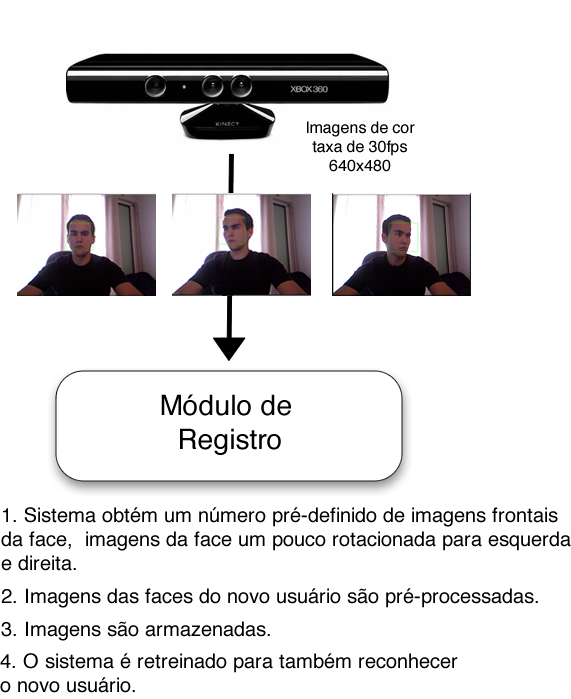
\includegraphics[scale=2.5]{figuras/4.ProblemaEProposta/registro.png}
			\end{center}
			\caption{Etapas de cadastro de um novo usuário no sistema.}
			\label{fig:registro}
		\end{figure}		

		\begin{enumerate}
			\item O novo usuário fica em uma posição fixa e frontal em relação ao \textit{Kinect}. 
			\item O sistema obtém um número pré-definido de imagens frontais do usuário.
			\item O usuário, então, deve rotacionar um pouco a face para a esquerda e o sistema obtém um número pré-definido de imagens do usuário. Depois, deve rotacionar um pouco para direita e o sistema obtém mais imagens do usuário.
			\item As imagens obtidas são processadas: as imagens são convertidas em escala de cinza, novas imagens são criadas recortando a região da face encontrada, as imagens, então, são redimensionadas e equalizadas criando assim uma padrão de tamanho, brilho e contraste nas imagens.
			\item Armazena-se as imagens.
			\item O sistema é treinado para, também, reconhecer esse usuário.
		\end{enumerate}

	Após o treinamento, o sistema \textit{True} reiniciará para que o reconhecimento seja feito utilizando as novas informações obtidas com o treinamento.
